\chapter{原子结构}

一百多年前,化学家们从实验中知道,物质是由分子组
成的,分子是由原子组成的,由于在化学反应中原子的种类和
数目不变,于是形成了原子是组成物质的最小微粒的概念.直
到十九世纪末,人们一直认为原子是不可再分的,但是随着物
理研究的深入和实验技术的提高,十九世纪末发现了一些新
的事实,证明原子是由更基本的微粒组成的.二十世纪以来,
物理学家们对原子和原子核的研究日益深人,建立了原子物
理和核物理的科学理论,在实际应用原子能方面也取得了很
大的进展,这一章和下一章我们就来学习原子结构和原子核
的初步知识.


\section{电子的发现}
\subsection{电子的发现}


原子不是不可再分的,而是由更小的微粒
组成的,这一认识是从发现电子开始的.

十九世纪后半期,科学家们在研究稀薄气体的放电时发
现,当玻璃管内的气体足够稀薄时,阴极就发出一种射线,这
种射线能使对着阴极的玻璃管壁发出荧光,叫做阴极射线.

英国科学家汤姆生(1856—1940)对阴极射线进行了一系
列的实验研究.1897年,他确认阴极射线是带负电的粒子.
汤姆生研究了阴极射线在电场和磁场中的偏转,根据测得的
数据计算出了这种带电粒子的荷质比$e/m$.
这种测定荷质比的
原理,我们在第一章中已经讲过,汤姆生发现,不同物质做成
的阴极发出的射线都有相同的
$e/m$
值.这表明不同物质都能发
射这种带电粒子,它是构成各种物质的共有成分.

汤姆生测得的阴极射线粒子的荷质比,大约是当时已知
的氢离子的荷质比的二千倍,汤姆生认为,这可能是由于阴
极射线粒子的电荷$e$很大,或者是它的质量$m$很小.后来汤
姆生测量了氢离子和阴极射线粒子的电荷,虽然测量不很准
确,但是足以证明阴极射线粒子的电荷与氢离子的电荷大小
基本上是相同的.由此得出结论,阴极射线粒子的质量比氢离
子的质量小得多:后来人们逐渐把这种粒子叫做电子.汤姆
生对证实电子的存在有很大的功劳,因而公认他是电子的发
现者.以后,美国科学家密立根又精确地测定了电子的电量,
这样由电子的荷质比和电量就可以算出电子的质量.

氢原子是当时已知的质量最小的原子,由电子的质量比
氢离子的质量小得多,汤姆生认为,电子可能是组成原子的基
本部分.

汤姆生发现电子,是物理学史上的重要事件.由于电子
的发现,人们认识到原子不是组成物质的最小微粒,原子本身
也具有结构,此后,围绕着原子结构的问题,原子物理以飞跃
的速度发展,人们对物质结构的认识进入了一个新时代.

\subsection{汤姆生的原子模型}

我们知道,物质在通常情况下是不带电的,因此,原子应该是电中性的,而电子是带负电的,如
果电子是原子的组成部分,那么原子里一定还有带正电的部
分.电子的质量很小,所以原子的质量应该主要集中在带正
电的部分.原子中带正电的部分和带负电的电子是怎样组成
原子的呢?这是物理学家们关心的一个问题.

在二十世纪的前十年里,科学家们提出了几种原子模型,
其中最有影响的是汤姆生提出的原子模型.在这个模型里,
原子被认为是一个球体,正电荷均匀分布在整个球内,电子则
象枣糕里的枣子那样镶嵌在球
内(图8.1),原子受到激发以后,电子开始振动发光,产生原子光谱.汤姆生的原子模型能
够解释一些实验事实,但是没过几年就被卢瑟福发现的新的实验事实否定了.
\begin{figure}[htp]
    \centering
    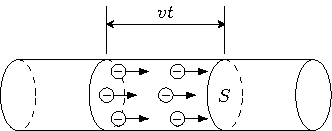
\includegraphics{fig/8-1.pdf}
    \caption{汤姆生的原子模型}
\end{figure}

\section{原子的核式结构的发现}
\subsection{$\alpha$粒子的散射和卢瑟福的原子核式结构模型} 

为了探测
原子内电荷的分布,在二十世纪的头十年里,发展了一种实
验方法:用各种粒子——X射线、电子和$\alpha$粒子轰击很薄的物
质层,通过观察这些粒子穿过物质层后的偏转情况,获得原
子结构的信息.这种实验叫做散射实验.那时候人们已经知
道,$\alpha$粒子是一种带正电荷的重粒子,它的电量是电子电量的
二倍,它的质量大约是电子质量的7300倍.某些放射性元素
放出的$\alpha$粒子具有很大的动能,可以当作轰击粒子,1909年
到1911年,在英国物理学家卢瑟福(1871—1937)指导下,
他的合作者们做了用$\alpha$粒子轰击金箔的实验,获得了重要的
发现.

实验的做法如下:在一个小铅盒里放有少量的放射性元
素钋,它发出的$\alpha$粒子从铅盒的小孔射出,形成很细的一束射
线射到金箔上.$\alpha$粒子穿过金箔后,打到荧光屏上产生一个
个的闪光,这些闪光可以用显微镜观察到.整个装置放在一
个抽成真空的容器里,荧光屏和显微镜能够围绕金箔在一个
圆周上转动(图8.2),从而可以观察到穿过金箔后偏转角度
不同的$\alpha$粒子.
\begin{figure}[htp]
    \centering
    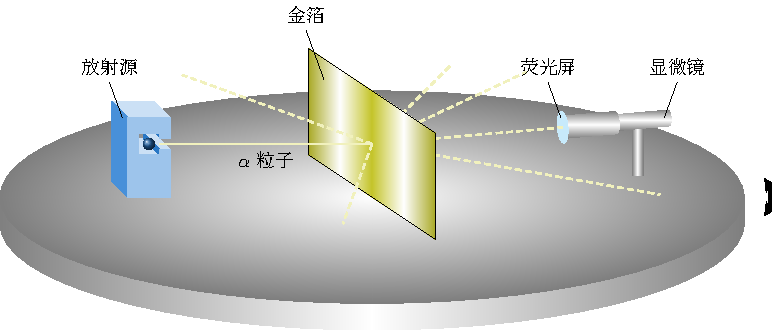
\includegraphics{fig/8-2.pdf}
    \caption{$\alpha$粒子散射实验装置示意图}
\end{figure}

实验表明,绝大多数$\alpha$粒子穿过金箔后仍沿原来的方向
前进,但是有少数$\alpha$粒子却发生了较大的偏转,并且有极少数
$\alpha$粒子的偏转超过了$90^{\circ}$,有的甚至几乎达到$180^{\circ}$,象是被金
箔弹了回来,这就是$\alpha$粒子的散射实验.

$\alpha$粒子的大角度散射现象,是出人预料的.因为根据汤
姆生原子模型的计算,$\alpha$粒子穿过金箔后的偏转最大不超过
零点几度,这是因为电子的质量很小,比$\alpha$粒子的质量小得
多,$\alpha$粒子碰到金箔原子内的电子,就象飞行的子弹碰到尘埃
一样,运动方向不会发生明显的改变,正电荷在原子内又是
均匀分布的,x粒子穿过原子时,它受到两侧正电荷的斥力有
相当大一部分互相抵消,因而使$\alpha$粒子偏转的力不会很大.

卢瑟福对$\alpha$粒子散射实验的结果进行了分析,得出结论,
除非原子的几乎全部质量和正电荷都集中在原子中心的一个
很小的核上,否则,$\alpha$粒子的大角度散射是不可能的.由此,
卢瑟福提出了他的原子核式结构模型:\textit{在原子的中心有一个
很小的核,叫做原子核,原子的全部正电荷和几乎全部质量都
集中在原子核里,带负电的电子在核外空间里绕着核旋转}.

按照这个学说,$\alpha$粒子穿过原子时,电子对$\alpha$粒子运动的
影响很小,影响$\alpha$粒子运动的主要是原子核.如果离核较远,
受到的库仑斥力就很小,运动方向也就改变很小.只有当$\alpha$粒
子与核十分接近时,才会受到很大的库仑斥力,发生大角度的
偏转(图8.3).由于原子核很小,$\alpha$粒子十分接近它的机会
很少,所以绝大多数$\alpha$粒子基本上仍按直线方向前进,只有极
少数发生大角度的偏转.
\begin{figure}[htp]
    \centering
    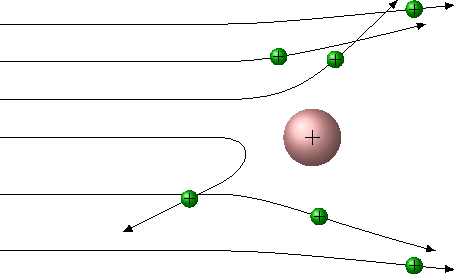
\includegraphics{fig/8-3.pdf}
    \caption{$\alpha$粒子十分接近原子核时才会发生大角度偏转}
\end{figure}


\subsection{原子核的电荷和大小} 

根据卢瑟福的原子核式结构模
型,可以推导出$\alpha$粒子的散射公式,利用这个公式和不同元素
对$\alpha$粒子散射的实验数据,可以计算出各种元素原子核的电
荷$Q$.当时测得碳的电荷$Q=6e$,铝的$Q=13e$或$14e$,金的
$Q=78e$或$79e$,其中$e$是基本电荷.原子核的电荷是研究原
子的重要资料,因为知道了某一元素原子核的电荷数,根据原
子是电中性的,就可以推算出这种原子内含有的电子数.当时
人们还注意到,测出的各种元素的原子核的电荷数,或者说元
素原子内的电子数,非常接近于它们的原子序数.这为深入
理解元素周期表提供了重要的线索,它说明元素周期表是按
原子中的电子数来排列元素的.

从$\alpha$粒子散射实验的数据还可以估计出原子核的大小.
因为知道了$\alpha$粒子的初动能和核电荷,就可以计算出$\alpha$粒子
跟原子核发生对心碰撞时可能达到的离原子核的最小距离
(这时$\alpha$粒子的动能完全转化为核电场中的电势能).这个最
小距离可以达到$10^{-14}$米.可见原子核的大小应在$10^{-14}$米
以下,原子半径大约是$10^{-10}$米,所以原子核的半径只相当于
原子半径的万分之一,原子核的体积只相当于原子体积的万
亿分之一.如果把原子比作直径等于100米的大球,那么原
子核只相当于直径为1厘米的一个小石子.原子核虽小,却
集中着原子的几乎全部质量,因此原子核的密度非常大,如
果1立方厘米的体积中完全充满原子核,那么它的质量将有
$10^7$吨!

\subsection*{练习一}
\begin{enumerate}
    \item $\alpha$粒子被原子散射的原因是什么?
    \item 卢瑟福的原子模型与汤姆生的原子模型,主要区别
    是什么?
    \item $\alpha$粒子的质量大约是电子质量的7300倍.如果$\alpha$
    粒子以速度$v$跟电子发生弹性正碰(假定电子原来是静止
    的),求碰撞后$\alpha$粒子的速度变化了多少,并由此说明,为什
    么原子中的电子不能使$\alpha$粒子发生明显的偏转.
    \item 已知氢原子的半径是$0.53\x10^{-10}$米,电子不致被吸
    引到核上,按照卢瑟福的原子模型,电子绕核做匀速圆周运动
    的速度和频率各是多大?
    \item 为什么在计算电子与核之间的引力作用时,可以不
    考虑万有引力?

\end{enumerate}

\section{玻尔的原子理论}
卢瑟福的原子核式结构学说很好地解释了$\alpha$粒子的散射
实验,初步建立了原子结构的正确图景,但跟经典的电磁理论
发生了矛盾.原来,电子没有被库仑力吸引到核上,它一定是
以很大的速度绕核运动,这种绕核运动是有加速度的.按照
经典电磁理论,做加速运动的电荷应该辐射出电磁波,因此它
的能量要逐渐减少.随着能量的减少,电子绕核运行的轨道
半径也要减小,于是电子将沿着螺旋线的轨道落入原子核,就
象绕地球运行的人造卫星受到上层大气阻力不断损失能量后
要落到地面上一样.这样看来,原子应当是不稳定的,然而实
际上并不是这样.同时,按照经典电磁理论,电子绕核运行时
辐射电磁波的频率应该等于电子绕核运行的频率,随着运行
轨道半径的不断变化,电子绕核运行的频率要不断变化,因此
原子辐射电磁波的频率也要不断变化.这样,大量原子发光
的光谱就应该是包含一切频率的连续光谱,然而实际上原子
光谱是由一些不连续的亮线组成的明线光谱.

这些矛盾表明,从宏观现象总结出来的经典电磁理论不
适用于原子这样小的物体产生的微观现象.

\subsection{玻尔的原子理论} 

为了解决上述矛盾,1913年丹麦青年
物理学家玻尔(1885—1962)在卢瑟福学说的基础上,把普朗
克的量子理论运用到原子系统上,提出了新的原子理论,在
原子物理的研究上迈出了重要的一步.玻尔原子理论的主要
内容是如下的假设:

一、原子只能处于一系列不连续的能量状态中,在这些
状态中原子是稳定的,电子虽然做加速运动,但并不向外辐射
能量、这些状态叫做\textbf{定态}.

二、原子从一种定态(设能量为$E_2$)跃迁到另一种定态
(设能量为$E_1$)时,它辐射或吸收一定频率的光子,光子的能
量由这两种定态的能量差决定,即
\[h\nu=E_2-E_1\]

三、原子的不同能量状态对应于电子的不同运行轨道.
由于原子的能量状态是不连续的,因此电子的可能轨道也是
不连续的,即电子不能在任意半径的轨道上运行.只有满足下
列条件的轨道才是可能的:轨道半径$r$跟电子的动量$mv$的
乘积等于 $h/2\pi$的整数倍,即
\[mvr=n\frac{h}{2\pi},\qquad n=1,2,3,\ldots\]
式中的$n$是正整数,叫做\textbf{量子数}.这种现象叫做\textbf{轨道的量
子化}.

玻尔把量子观念引入原子理论中,这是一个创举.根据
玻尔的假设,电子只能在某些可能的轨道上运动,电子在这些
道上运动时不辐射能量,处于定态,只有电子从一条轨道跃
迁到另一条轨道上时才辐射能量,辐射的能量是一份一份的,
等于这两个定态的能量差.这些就是玻尔理论的主要内容.

\subsection{氢原子的大小和能级}

玻尔在上述假设的基础上,利用
经典电磁理论和牛顿力学,对结构最简单的氢原子(只有一个
电子)进行了计算,算出了氢的电子的各条可能轨道的半径和
电子在各条轨道上运动时的能量(包括动能和电势能).玻尔
的计算结果可概括为两个公式:
\[\begin{cases}
    r_n=n^2 r_1\\
    E_n=\dfrac{1}{n^2}E_1
\end{cases}\qquad n=1,2,3,\ldots\]
式中的$r_1$代表第一条(即离核最近的一条)可能轨道的半径,
$E_1$代表电子在第一条轨道上运动时的能量,$r_n$、$E_n$分别代表
第$n$条可能轨道的半径和电子在第$n$条轨道上运动时的能
量,$n$是量子数.玻尔计算出$r_1$的值为$0.53\x10^{-10}$米,与过
去用其他方法计算出的氢原子的半径非常符合,玻尔计算出
$E_1$的值为$-13.6$电子伏.(计算中取离核无限远处的电势能为
零,电子带负电,在正电荷的场中电势能为负值;电子的动能
等于电势能绝对值的一半,所以总能量为负值.)

氢原子的各个定态的能量值,叫做它的\textbf{能级}.上面的计
算$E_n$的式子就是氢原子的能级公式,已知$E_1=-13.6$电子
伏,把$E_1$的值代入能级公式中,可以计算出氢原子各能级的
值:$n=2$时,$E_2=-3.4$电子伏;$n=3$时,$E_3=-1.51$电子伏;
$n=4$时,$E_4=-0.85$电子伏……可以看出,氢原子各个能级
的能量是不连续的,这种现象叫做\textbf{能量的量子化}.

在正常状态下,原子处于最低能级,这时电子在离核最近
的轨道上运动,这种定态叫做基态,给物体加热或有光照射
物体时,物体中的某些原子能够从相互碰撞或从人射光子中
吸收一定的能量,从基态跃迁到较高能级,这时电子在离核较
远的轨道上运动,这些定态叫做\textbf{激发态}.原子从基态向激发
态跃迁的过程,是吸收能量的过程,原子从较高的激发态面
较低的激发态或基态跃迁的过程,是辐射能量的过程,这个能
量以光子的形式辐射出去,这就是原子发光现象.原子无论
吸收能量或辐射能量,这个能量都不是任意的,而是等于原子
发生跃迁的两个能级间的能量差.


\subsection*{练习二}

\begin{enumerate}
    \item 利用公式$r_n=n^2r_1$和$E_n=E_1/n^2$,
计算氢原子的第2、3、4轨道的半径和电子在这些轨道上的能量.
\item 根据上题算出的结果,说明要把基态的氢原子激发
到$n=2$的能级上去,需要供给电子多大的能量.如果用电磁
波来供给这个能量,需要用波长多长的电磁波?这个波长属于
哪个波段?
\end{enumerate}

\section{玻尔原子理论对氢光谱的解释}

玻尔理论的成功主要表现在对氢光谱规律的解释上.

\subsection{氢光谱的规律}

人们很早就发现每种元素都发出自己独
特的光谱,各种元素的每条光谱线的频率都是固定不变的,在
所有的光谱中,人们对氢光谱研究得最清楚,氢光谱在可见光
区内有四条谱线,这四条谱线叫做$H_{\alpha}$、$H_{\beta}$、$H_{\gamma}$、$H_{\delta}$.它们的波
长分别是
\begin{center}
    \begin{tabular}{cc}
        $H_{\alpha}$  &0.6562微米\\
        $H_{\beta}$  &0.4861微米\\
        $H_{\gamma}$  &0.4340微米\\
        $H_{\delta}$  &0.4101微米\\
    \end{tabular}
\end{center}

1885年瑞士的中学教师巴耳末(1825—1898)研究了这
些波长之间的关系,发现了它们之间的关系可以用一个公式
来表示.如果利用波长的倒数$1/\lambda$,
巴耳末的公式可写作
\[\frac{1}{\lambda}=R\qty(\frac{1}{2^2}-\frac{1}{n^2}),\qquad n=3,4,5,\ldots\]
式中的$R$是一个常数,叫做\textbf{里德伯恒量},实验测得$R$的值为
$1.096776\x10^7{\rm m^{-1}}$.

上面的公式叫做\textbf{巴耳末公式}.当$n=3,4,5,6$时,用这个公
式计算出的四条光谱线的波长跟上面从实验测得的$H_{\alpha}$、$H_{\beta}$、$H_{\gamma}$、$H_{\delta}$四条谱线的波长符合得非常好,于是人们把氢光谱的
这一系列谱线叫做巴耳末系.巴耳末公式反映了氢光谱这一
系列谱线的规律性.

\subsection{玻尔原子理论对氢光谱规律的解释} 

按照玻尔原子理
论,原子从较高能级 $E_2$跃迁到较低能级$E_1$时,辐射出的光子
能量为$k\nu =E_2-E_1$.因此,氢原子的电子从能量较高的轨道$n$
跃迁到能量较低的轨道2时,辐射出的光子能量应为$h\nu=E_n-E_2$.
利用第三节中氢原子的能级公式,可得
\[E_n=\frac{E_1}{n^2},\qquad E_2=\frac{E_1}{2^2} \]
由此可得\[h\nu=-E_1\qty( \frac{1}{2^2}-\frac{1}{n^2} )\]
由于$\nu=c/\lambda$,
所以上式可写作
\[\frac{1}{\lambda}=\frac{-E_1}{hc}\qty( \frac{1}{2^2}-\frac{1}{n^2})\]
把这个式子与前面的巴耳末公式相比较,可以看出它们的形
式是完全一样的,并且$R=-E_1/(hc)$
计算出$-E_1/(hc)$
的值为$1.097373\x10^7{\rm m^{-1}}$,与前面给出的的实验值符合得很好.这就是说,
根据玻尔理论,不但可以推导出表示氢光谱的规律性的公式,
而且还可以从理论上来计算里德伯恒量的值.

由此可知,氢光谱的巴耳末系是电子从$n=3,4,5,6$等能
级跃迁到$n=2$的能级时辐射出来的.

玻尔理论不但成功地解释了氢光谱的巴耳末系,而且对
当时已发现的氢光谱的另一线系——帕邢系(在红外区)也能
很好地解释.它是电子从$n=4,5,6$等能级向$n=3$的能级跃
迁时辐射出来的.此外,玻尔理论还预言了当时尚未发现的
氢原子的其他光谱线系,这些线系后来相继被发现,也都跟玻
尔理论的预言相符.其中赖曼系在紫外区,是电子从$n=2,
3,4$等能级向$n=1$的能级跃迁时发出的;布喇开系在远红外
区,是电子从$n=5,6,7$等能级向$n=4$的能级跃迁时发出的.
图8.4和8.5分别是用氢原子的能级图和轨道图表示的各线
系的情况.
\begin{figure}[htp]
    \centering
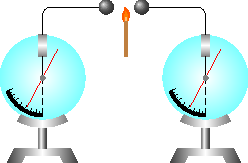
\includegraphics[scale=1]{FIG/8-4.pdf}
    \caption{氢原子的能级图}
\end{figure}

\begin{figure}
    \centering
    \begin{tikzpicture}[scale=1.6, >=stealth]
        \draw (0,0) circle (5pt);
        \draw (0,0) circle (15pt);
        \draw (0,0) circle (30pt);
        \draw (0,0) circle (50pt);
        \draw (0,0) circle (75pt);
        \draw (0,0) circle (100pt);
    \fill (0,0) circle (1.5pt);

    \node at (0,-5pt-1.4) {$n=1$};
    \node at (0,-15pt-1.4) {$n=2$};
    \node at (0,-30pt-1.4) {$n=3$};
    \node at (0,-50pt-1.4) {$n=4$};
    \node at (0,-75pt-1.4) {$n=5$};
    \node at (0,-100pt-1.4) {$n=6$};
    
    
    \node at (50:50pt) {赖曼系(紫外线)};
    \node at (0:50pt) {巴耳末系};
    \node at (-25:70pt) {帕邢系(红外线)};
    \node at (-45:85pt) {布喇开系};
    \node at (-60:95pt) {逢德系};
    
    
    
    
    \draw[->] (60:100pt)--(60:5pt);
    \draw[->] (55:75pt)--(55:5pt);
    \draw[->] (50:50pt)--(50:5pt);
    \draw[->] (45:30pt)--(45:5pt);
    \draw[->] (40:15pt)--(40:5pt);
    
    \draw[->] (10:100pt)--(10:15pt);
    \draw[->] (5:75pt)--(5:15pt);
    \draw[->] (0:50pt)--(0:15pt);
    \draw[->] (-5:30pt)--(-5:15pt);
    
    \draw[->] (-20:100pt)--(-20:30pt);
    \draw[->] (-25:75pt)--(-25:30pt);
    \draw[->] (-30:50pt)--(-30:30pt);
    
    \draw[->] (-45:100pt)--(-45:50pt);
    \draw[->] (-50:75pt)--(-50:50pt);
    
    \draw[->] (-60:100pt)--(-60:75pt);
    
    
    \end{tikzpicture}
    \caption{氢原子的轨道图}
\end{figure}

    \section*{阅读材料:定态存在的实验证明——夫兰克-赫兹实验}
    玻尔原子理论的一个重要假设是原子存在着某些分立的
    能态,各能态之间有一定的间隔.玻尔的这一假设能从实验
    中观察到吗?1914年,也就是玻尔原子理论提出后的第二年,
    由德国物理学家夫兰克(1882—1964)和赫兹所做的著名实
    验,证实了原子分立能态的存在,为玻尔假设提供了有力的证
    据.

    夫兰克-赫兹实验的方法是,使电子通过压强很低的汞蒸
    气,测量电子与汞原子碰撞前后损失的能量,同时测定汞原子
    在这些碰撞中获得的能量.夫兰克和赫兹发现,当电子以较
    小的动能碰撞汞原子时,电子通过汞蒸气后的能量几乎完全
    不变.这个结果可以这样来解释:汞原子的质量是电子质量
    的几十万倍,当电子的动能较小时,跟汞原子的碰撞是弹性碰
    撞,汞原子只吸收电子的极小一部分动能,电子几乎不损失动
    能.

    但是当电子的动能增加到5电子伏时,实验结果发生明
    显的变化,这时电子与汞原子碰撞时,几乎准确地损失4.9电
    子伏的能量.当电子的动能增加到6电子伏时,电子与汞原
    子碰撞也仍然只损失4.9电子伏的能量.这表明,汞原子不
    能吸收小于4.9电子伏的能量;当提供的能量比4.9电子伏稍
    微多一点时,它也仍然只接受4.9电子伏.由此可以认为,汞原
    子有一个比它的最低能态大4.9电子伏能量的定态.在这个
    能态和最低能态之间不存在其他的能态.

    按照玻尔原子理论,汞原子在吸收了4.9电子伏的能量
    后,将从最低能态跃迁到较高能态;当电子从较高能态跃迁回
    低能态时,应辐射出光子,而且辐射出的光子的能量应等于原
    来跃迁到较高能态时吸收的能量,即4.9电子伏.夫兰克和
    赫兹在实验中果然找到了被激发的汞原子辐射出的这一光谱
    线,其波长为2537埃,它的能量恰好是4.9电子伏.这表明,
    汞原子和电子碰撞时,确实获得了4.9电子伏的能量.

    夫兰克和赫兹在以后的实验中还发现,被电子碰撞的汞
    原子也能获得其他确定的能量,例如6.7电子伏、10.4电子
伏,这相当于把汞原子激发到更高的能态.在每一种情况下,
汞原子都辐射出相应能量的光谱线,这样就用实验证明了玻
尔关于原子存在着不连续能态的假设是正确的.


\subsection*{练习三}
\begin{enumerate}
    \item 根据玻尔理论,$H_{\alpha}$、$H_{\beta}$谱线光子的能量应该是多少
电子伏?根据实验测得的$H_{\alpha}$、$H_{\beta}$的波长算得的光子的能量是
多少电子伏?二者是否一致?
\item 计算氢原子从$n=4$,$n=5$能级分别跃迁到$n=3$能
级时辐射出的光子的波长.这两条谱线在哪个波段?它们属
于哪个线系?
\item 怎样用玻尔原子理论解释原子吸收光谱的规律?
\end{enumerate}


\section{玻尔原子理论的困难和量子力学}

玻尔原子理论在解释核外只有一个电子的氢光谱上很成
功;但是用来解释具有两个以上电子的比较复杂的原子光谱
时却遇到了困难,理论推导出来的结论跟实验事实出入很大.
玻尔和其他物理学家研究了这个问题,终于明白这个理论成
功之处在于它引入了量子观念,失败之处在于它保留了过多
的经典物理理论.

到本世纪二十年代,大约在玻尔原子理论建立十年之后,
海森堡(1901—1976)、薛定谔(1887—1961)、玻尔、玻恩(1882
—1969)、狄拉克(1902—1984)等物理学家在量子观念的基础上
建立了量子力学.开始,海森堡和薛定谔互相独立地提出了
数学表达形式不同的理论,后来薛定谔很快就证明了这两种
理论是完全等价的.是对同一事物的两种描述方式,薛定谔的
理论更接近德布罗意的物质波的观念,也常常称为波动力学.
薛定谔力图用数学形式来描述物质的波粒二象性.他从麦克
斯韦的光的电磁学说得到启发,认为电子的德布罗意波也
可以用类似于光波的方式来描述,于是写出了描述物质波的
方程,这就是著名的薛定谔方程.这个方程既描述了电子的
物质波的行为,又含有电子的粒子性的特征.可惜由于我们
的数学知识不足,在这里还不能写出这个方程并予以讨论.
从解薛定谔方程得到的结果,不但成功地解释了玻尔原子理
论所能解释的现象,而且能够解释大量的玻尔理论所不能解
释的现象.我们在前面提到的玻尔理论的基本假设,在量子
力学里变成了从理论上推导出来的必然结果,而不再是人为
的假设了.原来,在薛定谔方程中,只有原子中的电子具有某
些不连续的能量值时,这个方程才有解.由薛定谔方程的解
中得出的氢原子中电子能量的可能值,正好就是由玻尔原子
理论给出的值.

建立在量子力学基础上的原子理论,核外的电子并没有
确定的轨道,从薛定谔方程的解我们只能知道,核外电子在原
子内各处出现的几率.氢原子在基态时,它的电子经常出现
的几率最大的区域是以原子核为中心的一个球壳,这个球壳
的半径为$0.53\x10^{-10}$米,这个数值跟用玻尔原子理论计算的
氢原子基态的轨道半径相同,可见,玻尔的电子轨道,只不
过是电子出现几率最大的地方.电子在核外的运动情况,通
常用“电子云”来形象地描述.这就是用小黑点的稠密与稀疏
来代表电子在核外各处出现的几率的大小,这样我们就可以
画出原子的电子云图,图中原子核好象是被一层云雾笼罩着,
云雾浓度大的地方,电子出现
的几率大,云雾浓度小的地方,
电子出现的几率小.于是电子
云的概念就代替了玻尔理论中
电子轨道的概念,图8.6是氢
原子基态的电子云.


量子力学出现以后,在说明原子结构方面迅速取得了巨
大的成功,很快地被物理学家所接受.现在它的应用已远远
超出原子结构的范围,成为物理学家研究微观世界的基本理
论工具.但是,量子力学虽然是原子世界的很成功的数学“模
型”,却不能给我们提供一个直观的物理图景.量子力学告诉
我们,既不可以把电子等微观粒子当成牛顿力学中的质点,也
不可以把物质波当成我们熟悉的机械波.由于在这里研究的
是比日常物体小得很多很多的微观客体,我们在日常经验中
所形成的一些概念在这里不再适用应该是很自然的事情.


\section{原子的受激辐射~~激光}
\subsection{自发辐射和受激辐射}

原子发光有两种情形,一种是自
发辐射,一种是受激辐射.处于激发态的原子是不稳定的,只
能停留很短的时间,通常约为$10^{-8}$秒,就自发地跃迁到较低
能级去,同时辐射出一个光子,光子的能量$h\nu =E_2-E_1$,其中
$E_2$和$E_1$分别代表原子处于高能级和低能级时的能量.这种辐
射叫做\textbf{自发辐射}.原子发生自发辐射时,各个原子发出的光
子是向四面八方辐射的,它们的频率、初相和偏振方向互不相
同,而且每个原子每次发光持续的时间很短,约$10^{-9}$秒,下
一次发光又会发出跟前一次不同的光子,因此这些光叠加时
不会产生稳定的干涉花样,看到的只是大量光产生的一种平
均效果,这种光就是自然光,这就是普通光源发光的情形.

原子发光还有一种情形,就是当原子处于激发态$E_2$时,
如果恰好有能量$h\nu =E_2-E_1$的光子从附近通过,在入射光子
的电磁场的影响下,原子会发出一个同样的光子而跃迁到低
能级$E_1$去,这种辐射叫做\textbf{受激辐射}.原子发生受激辐射时,发
出的光子的频率、发射方向、初相和偏振方向等,都跟入射光
子完全一样,也就是说,受激辐射的光子跟入射光子没有任何
区别.这样,一个入射光子由于引起受激辐射就变成了两个
同样的光子.如果这两个光子在媒质中传播时再引起其他原
子发生受激辐射,就会产生越来越多的相同的光子,使光得到
加强,这就是激光,也就是说,由于受激辐射而得到加强的光
就是\textbf{激光}.

但是,要实际产生激光并不容易,从1917年爱因斯坦从
理论上指出受激辐射到1960年世界上制成第一台激光器,经
过了四十多年的时间,这是因为,能量$h\nu =E_2-E_1$的光子从媒
质中通过时,既能引起处于$E_2$能级的原子发生受激辐射,使
光增强(也叫做光放大),也能使处于$E_1$能级的原子被激发而
跃迁到能级$E_2$,这时光子被吸收,使光减弱.在通常情况下,
处于低能级$E_1$的原子数大于处于高能级$E_2$的原子数,光吸
收过程胜过光放大过程,因而得不到激光.

应用量子力学研究了各种原子的能级后发现,某些原子
有一些特殊的能级,原子处在这些特殊能级上时,虽然也是激
发态,却能停留较长的时间,比处在其他激发态的时间可长约
十万倍,因而不易发生自发跃迁.这种激发态叫做\textbf{亚稳态}.因
此,如果原子有两个激发态$E_2$和$E_1$,其中较高能级$E_2$是亚稳
态,而较低能级$E_1$是寿命很短的激发态,我们设法把处于基
态的原子大量 激发到亚稳态$E_2$,处于高能级$E_2$的原子数就
可以大大超过处于低能级$E_1$的原子数,这种状态叫做\textbf{粒子数
反转}.这时如果有能量等于$E_2-E_1$的光子从原子附近通过,
就会产生大量的受激辐射,于是光放大过程大于光吸收过程,
得到较强的激光.

能产生激光的装置,叫做激光器.现在激光器的种类已
达几百种,有固体激光器、液体激光器、气体激光器、半导体激
光器等多种类型,适用于不同的用途.

\subsection{激光的特点及应用}

激光的主要特点是亮度高、方向性
好、单色性好、相干性好、红宝石激光器产生的激光亮度比太
阳光的亮度要高几百亿倍.激光光束几乎是完全不发散的平
行光,方向性非常好,同一个激光器产生的激光的波长范围很
窄,接近于单一频率,单色性比其他光源发出的光都好,原子
发生受激辐射时发出的光子的频率、初相和偏振方向等都跟
人射光子完全一样,所以激光的相干性很好,正是由于激光
有这些突出的特点,所以在各个领域得到了广泛的应用.

激光的亮度高、能量集中,可以使物体的被照部分在不到
千分之一秒的时间内产生几千万度的高温.因此,工业上可
以利用激光束在硬质、难熔的材料上进行打孔、切割,还可以
用来焊接金属,不但提高工作效率,而且加工质量得到保证.
医学上用激光束作“手术刀”进行手术,出血量少,刀口愈合得
快.激光束可以聚焦到比针尖还小的范围内,手术的时间极
短,特别适宜于眼科手术.利用激光焊接脱落的视网膜、切除
虹膜等都非常成功.

激光的方向性好,能照射到很远的地方,因此用它来测量
距离是非常理想的,可以达到很高的精度,对准目标发出一
个极短时间的激光脉冲,然后测出激光从发出时刻到反射回
发射点经过的时间$t$,就可以按公式$\ell=\frac{1}{2}ct$求出激光从发
射点到被测目标的距离,式中的$c$是光速.用这种方法测量
月球上某点到地球上某点的距离,误差不超过几厘米.实际
上,按照这种原理设计制造的激光测距仪就是一种激光雷达.
多用途的激光雷达不仅可以测量距离,而且能够测定被测目
标的方位、运动速度、运动轨迹,甚至能描绘出目标的形状,进
行识别和自动跟踪.

利用激光单色性好、相干性好的特点,可以用光的干涉方
法来精确地测量长度,检查加工零件的质量,进行全息照相.

激光还可以用来辐照种子,培育良利,控制化学反应,用
于舞台布景等.

激光是二十世纪的重大发明之一,自1960年出现以来,
目前还处在迅速发展时期,激光在科学技术各个领域的应用,
有力地促进了这些领域的发展,并产生了一些新的边缘科学,
例如激光化学、激光生物学等.今后随着激光技术的发展,将
会促进一些重大应用的实,例如光纤激光通讯,激光核聚
变、激光分离同位素等,并将会出现一个新兴的工业部门-
激光工业.在未来的科技发展中,激光起着重要的作用.

\section*{复习题}

\begin{enumerate}
    \item 电子是怎样发现的?电子的发现对认识原子结构起了什么作用?
    \item 原子核是怎样发现的?卢瑟福的原子模型是什么样
的?怎样用卢瑟福的原子模型来解释$\alpha$粒子的大角度散射?
\item 卢瑟福原子模型的困难是什么?玻尔是怎样解决这
一困难的?根据玻尔的原子理论,原子的模型又是怎样的?
\item 写出氢原子的轨道半径公式和能级公式,说明式中
各量的意义.
\item 玻尔理论怎样成功地解释了氮原子光谱的规律?
\item 什么叫做受激辐射?怎样才能产生大量的受激辐
射,从而得到激光?激光有哪些主要的特点?举例说明激光的
应用.
\end{enumerate}


































